\section{Additional Stratified Error Plots}

\begin{figure*}[t]
  \centering
  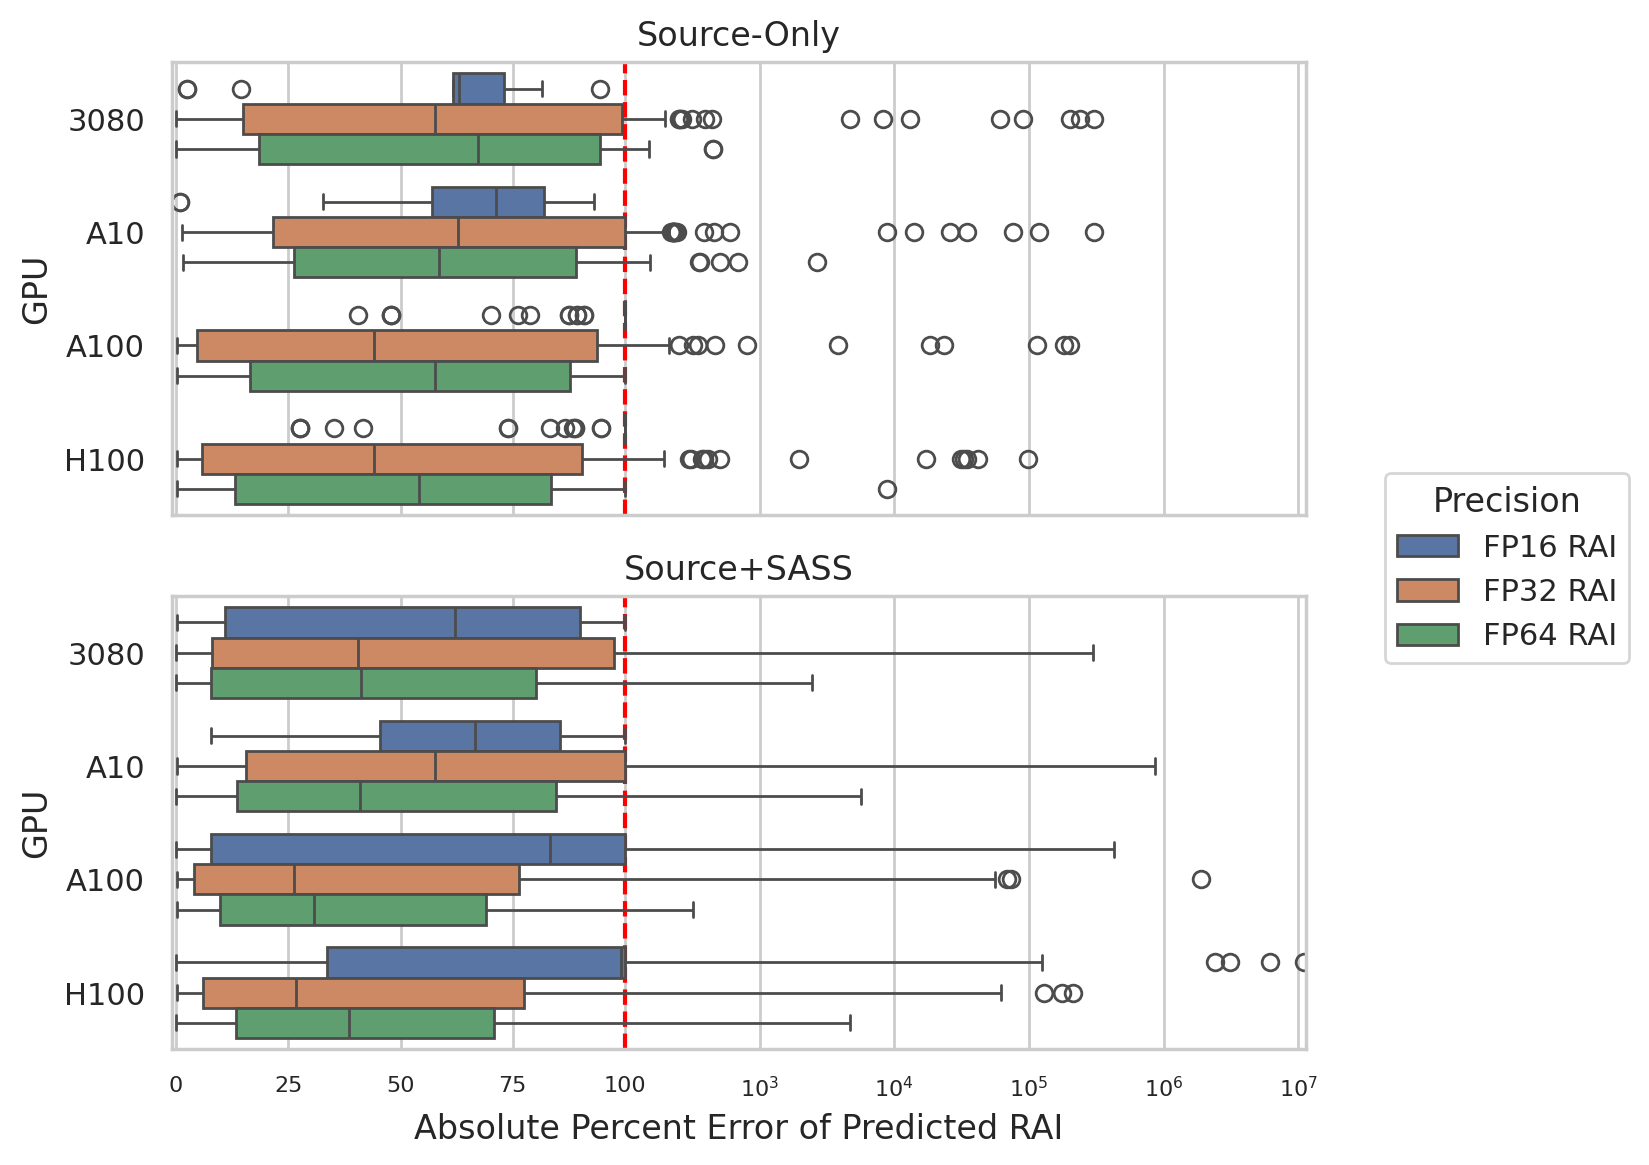
\includegraphics[width=\textwidth]{figures/ape_by_gpu.png}
  \caption{Absolute percent error on nonzero \rai cases, stratified by GPU.
  The smaller-cache 3080/A10 settings are generally less stable than A100/H100, especially for source-level reasoning about FP32/FP64 DRAM-visible traffic.}
  \Description{Stratified boxplots of nonzero arithmetic-intensity absolute percent error by GPU, showing noisier 3080 and A10 distributions than A100 and H100 in several FP32 and FP64 settings.}
  \label{fig:appendix-ape-by-gpu}
\end{figure*}

\begin{figure*}[t]
  \centering
  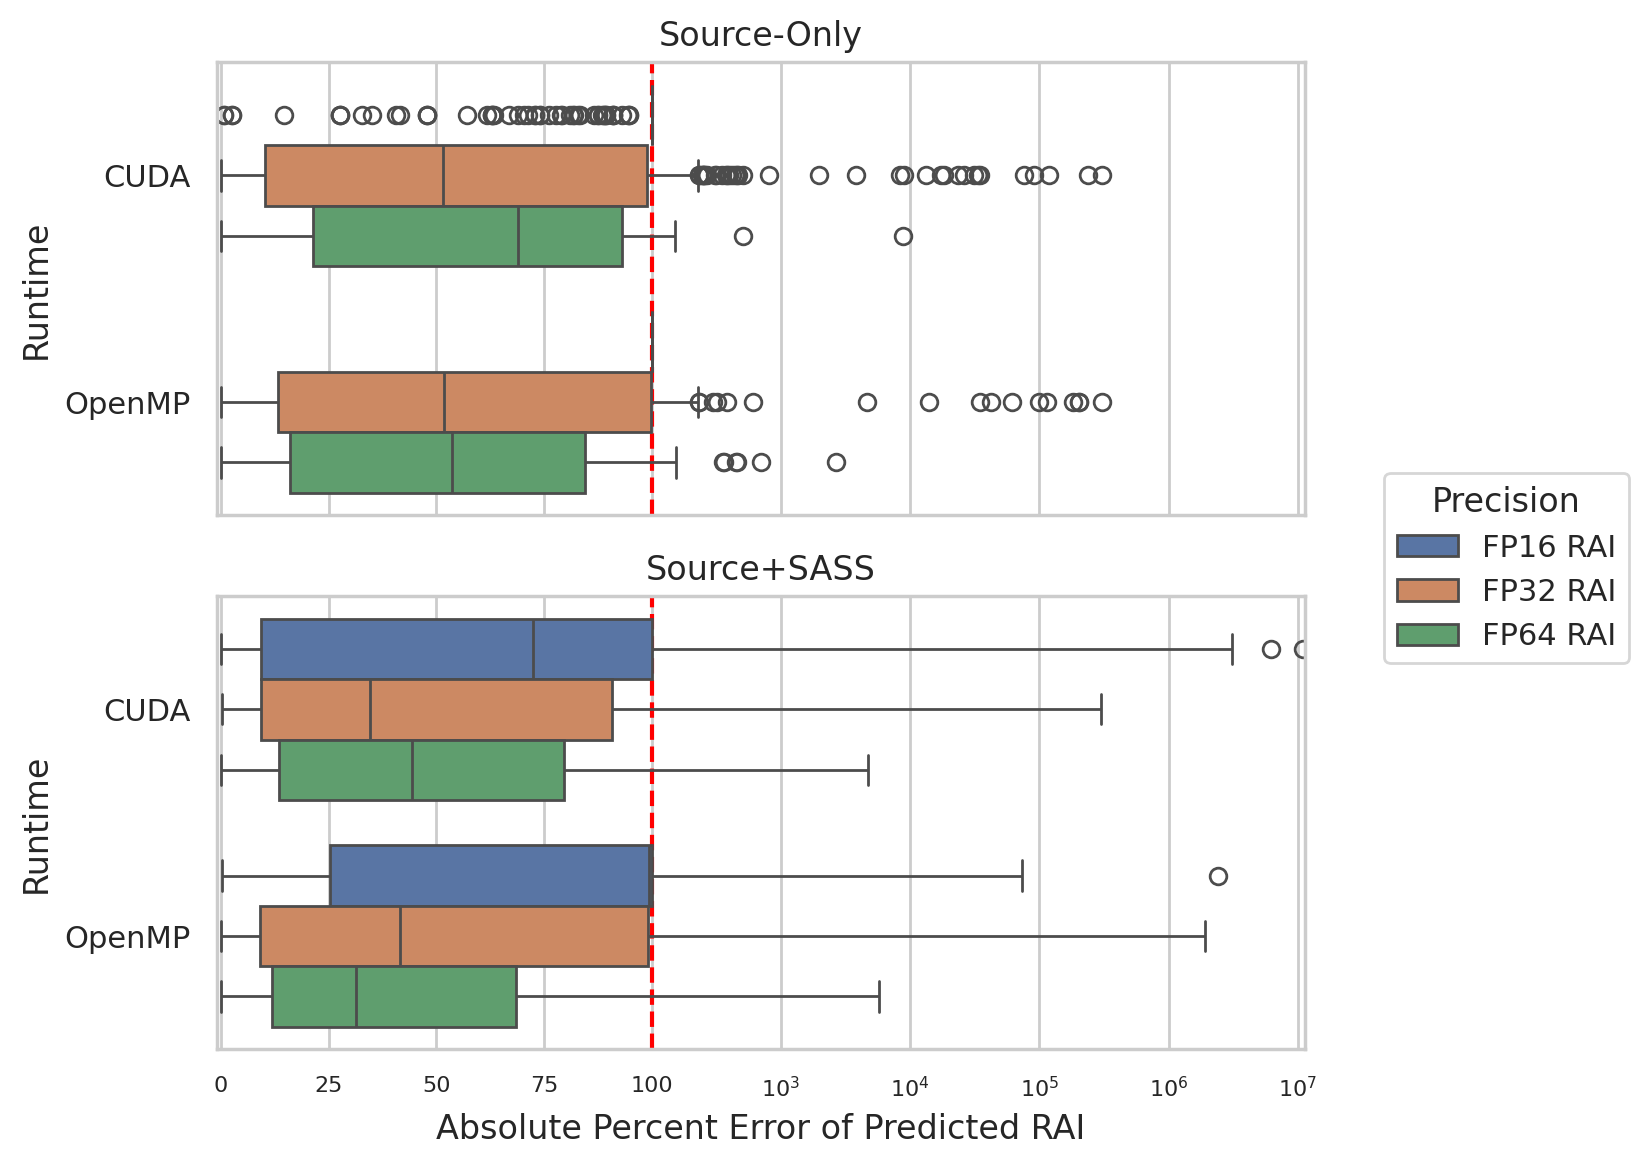
\includegraphics[width=\textwidth]{figures/ape_by_runtime.png}
  \caption{Absolute percent error on nonzero \rai cases, stratified by runtime.
  The runtime split is precision-sensitive rather than uniform: CUDA tends to be easier for FP16/FP32 triage, while FP64 remains mixed across CUDA and OpenMP.}
  \Description{Stratified boxplots of nonzero arithmetic-intensity absolute percent error by runtime, showing that CUDA is often easier than OpenMP for FP16 and FP32 while FP64 remains mixed.}
  \label{fig:appendix-ape-by-runtime}
\end{figure*}

\section{Illustrative Released Rows}

\begin{table*}[t]
  \centering
  \caption{Illustrative released samples used only for intuition, not as additional evaluation evidence. These examples show accurate numeric \rai predictions in regimes where the relevant computation and memory behavior are visible to the model.}
  \label{tab:illustrative-rows}
  \scriptsize
  \setlength{\tabcolsep}{4pt}
  \begin{tabular}{p{0.17\textwidth} p{0.20\textwidth} p{0.23\textwidth} p{0.32\textwidth}}
    Case & Released sample & Expected $\rightarrow$ predicted \rai & Why it matters \\
    \midrule
    Hidden lowered FP16 work &
    \texttt{accuracy-cuda}, A100, \opus &
    FP16 \sourceonly: 0.0254 $\rightarrow$ 0.0; FP16 \sourcesass: 0.0254 $\rightarrow$ 0.0256 &
    The source-only explanation notes that compiler-generated \texttt{HFMA2} materialization may exist but cannot be justified from source alone, so it conservatively predicts zero FP16 work. The SASS-backed explanation instead points to an executed \texttt{HFMA2.MMA} instruction on the taken path and counts it as real FP16 arithmetic. \\
    Source-visible FP32 work &
    \texttt{boxfilter-cuda}, A100, \opus &
    FP32 \sourceonly: 21.975 $\rightarrow$ 22.0 &
    The source already exposes the 21-tap loop trip count, the 64 output threads per block, and the roughly 1\,MiB unique read footprint. In this regime, source-only reasoning is already enough and post-compilation evidence adds little. \\
    Regular stencil-like FP32 work &
    \texttt{asmooth-cuda}, 3080, \opus &
    FP32 \sourceonly: 0.8329 $\rightarrow$ 0.8331 &
    The kernel has a regular source-visible arithmetic and memory pattern, so the model can infer a close DRAM-level ratio without SASS. \\
    Source/SASS-visible FP64 work &
    \texttt{burger-cuda}, 3080, \opus &
    FP64 \sourcesass: 2.9669 $\rightarrow$ 2.9684 &
    The double-precision arithmetic and global-memory structure are visible enough after lowering for the SASS-backed estimate to nearly match the profiler-derived \rai. \\
  \end{tabular}
\end{table*}


\section{Exploratory Failure Map}

\begin{figure*}[t]
  \centering
  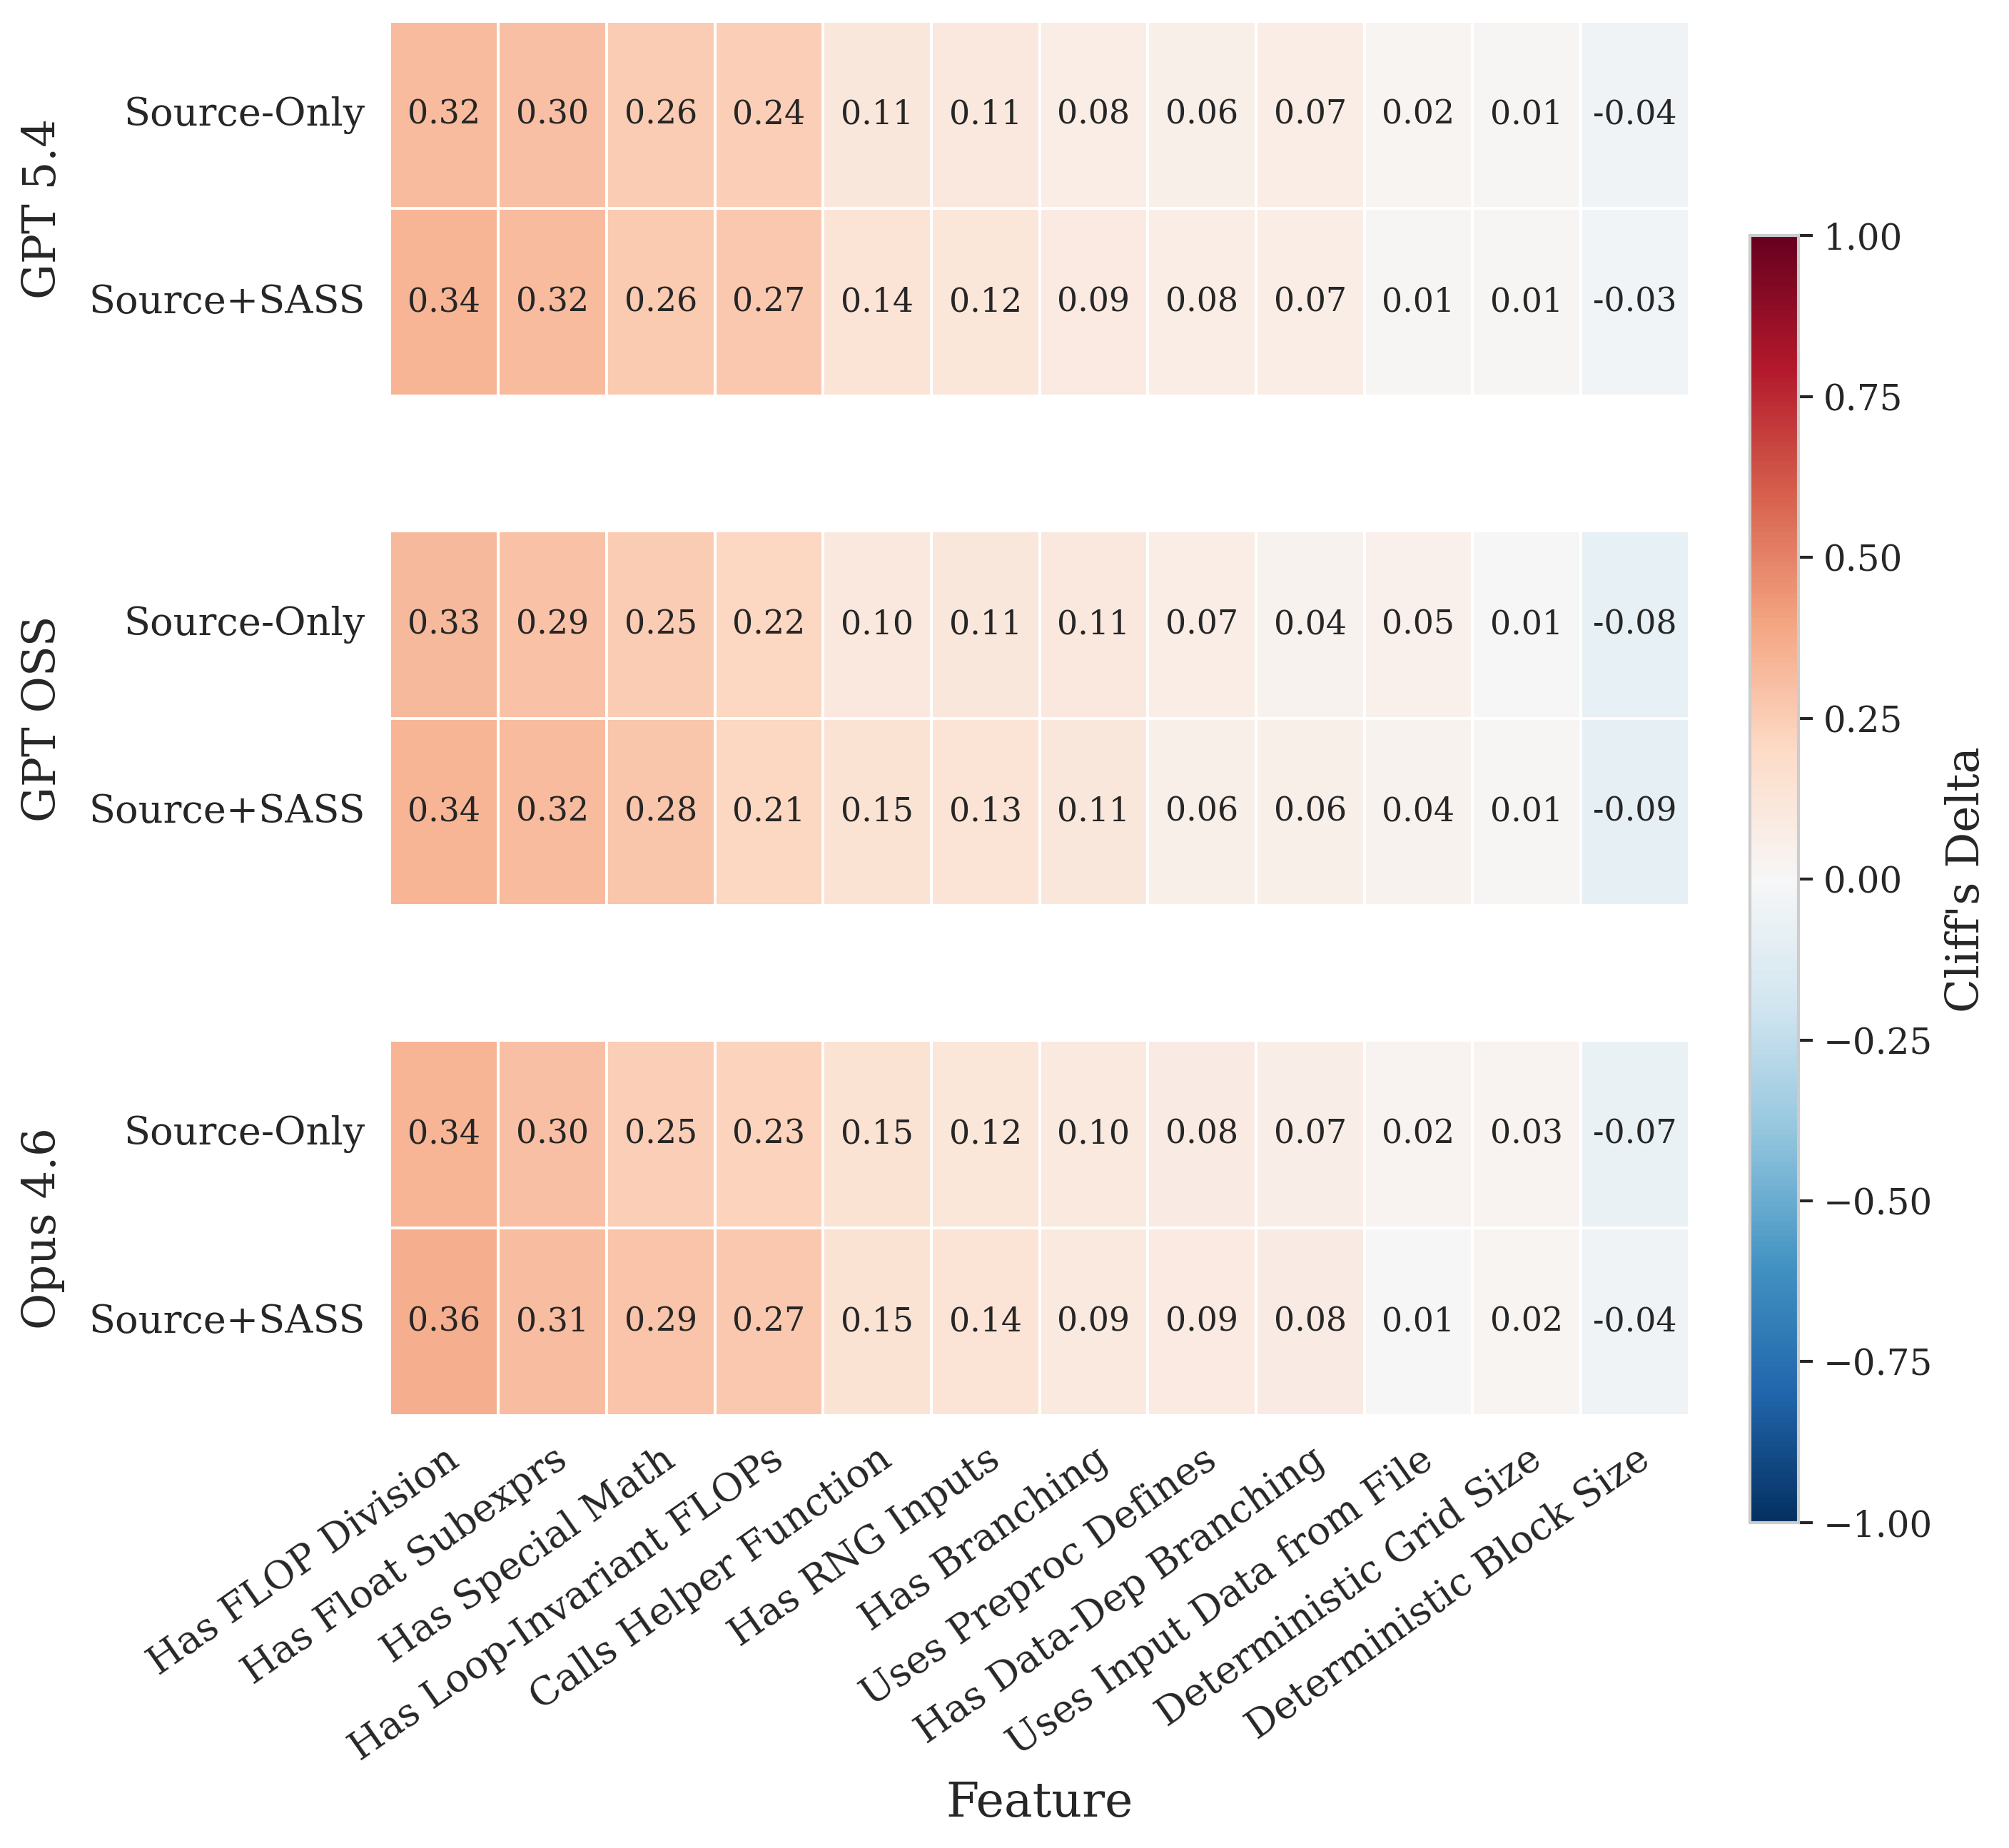
\includegraphics[width=\textwidth]{figures/feature_association_heatmap.png}
  \caption{Exploratory feature/error association heatmap from the released artifact.
  Positive Cliff's delta means higher absolute \rai error when the feature is present.
  The strongest repeated error signals come from division, special math, reusable subexpressions, and loop-invariant floating-point work.
  A post-hoc Mann--Whitney/BH sanity check across the same 72 model$\times$prompt$\times$feature cells preserves repeated positive associations for division, common float subexpressions, special math, loop-invariant FLOPs, helper-function calls, RNG inputs, branching, preprocessor defines, and data-dependent branching; those features appear in 7--90\% of the 1{,}336 voted kernels.
  Because the feature labels are generated by an auxiliary LLM-voting pipeline, we treat this figure as descriptive rather than causal.}
  \Description{A heatmap of exploratory feature associations with absolute arithmetic-intensity error, where darker positive cells cluster around division, transcendental math, reusable subexpressions, and loop-invariant floating-point work.}
  \label{fig:feature-heatmap}
\end{figure*}

\section{Repeated-Query Variability (Detailed)}
\label{sec:appendix-repeated-query}

\autoref{tab:repeated-query-variance} gives the per-precision detail behind the consistency results of RQ3 (\autoref{sec:results}): the coefficient of variation of predicted \rai and the \bandwidthbound/\computebound agreement rate across the four repeated queries, for each model and evidence setting on the 24-kernel panel of \autoref{sec:study-design}.
The panel is complete for \gptfivefour and partially complete for \gptoss; the \opus repeats are pending and will be added.

\begin{table*}[t]
  \centering
  \caption{Repeated-query response variability on the repeat-trials panel. ``CV'' is the median coefficient of variation of predicted \rai across repeats (lower is more consistent); ``Agr'' is the fraction of cells whose \bandwidthbound/\computebound call is unanimous across repeats. Computed at the main-paper decode settings.}
  \label{tab:repeated-query-variance}
  \scriptsize
  \setlength{\tabcolsep}{4pt}
  \begin{tabular}{llrrrrrr}
    \toprule
    & & \multicolumn{2}{c}{FP16} & \multicolumn{2}{c}{FP32} & \multicolumn{2}{c}{FP64} \\
    \cmidrule(lr){3-4}\cmidrule(lr){5-6}\cmidrule(lr){7-8}
    Model & Evidence & CV & Agr & CV & Agr & CV & Agr \\
    \midrule
    \texttt{GPT OSS} & source-only & 0.00 & 100\% & 0.27 & 81\% & 0.20 & 76\% \\
    \texttt{GPT OSS} & source+SASS & 0.00 & 95\% & 0.44 & 69\% & 0.49 & 62\% \\
    \bottomrule
  \end{tabular}
\end{table*}


\section{Reasoning versus Memorization Probe (Planned)}
\label{sec:appendix-contamination}

% PLACEHOLDER SECTION -- fill once the deferred perturbation experiment is run.
Because the corpus is public, some kernels may appear in pretraining data, so accurate predictions could reflect recall rather than reasoning.
We plan a \emph{cosmetic} perturbation probe that renames kernel and function identifiers and strips comments while leaving the computation, and therefore the ground-truth \rai, unchanged.
A model that reasons from program structure should be largely invariant to these edits, whereas a model leaning on memorized identifiers or familiar source text should degrade.
Because cosmetic edits do not change the ground truth, this probe needs no re-profiling and no target-hardware access, which is essential because the original profiling GPUs are no longer available to us.
We will report the change in \bandwidthbound/\computebound classification accuracy and \rai error between original and cosmetically perturbed kernels.

\section{Anonymity Note}

The current workspace contains public website and repository mirrors for the dataset artifact.
To preserve double anonymity, the manuscript omits those URLs.
The project README records the replacement points for a de-anonymized camera-ready version.
